\documentclass[12pt]{report}
\usepackage{graphicx}
\usepackage[utf8]{vietnam}
\usepackage[left=3cm, right=3cm, top=3cm, bottom =3cm]{geometry}
\usepackage{pdfpages}
\usepackage{fancyhdr}
\usepackage{hyperref}
\usepackage{etoolbox}

% \setcounter{tocdepth}{4}

% Link color setup
\hypersetup{
	colorlinks = true,
	linkcolor = black,
	citecolor = blue
}

% Change format of page
\pagestyle{fancy}
\fancyhf{}
\fancyhead{}
\fancyfoot{}
\fancyhead[L]{Hệ điều hành}
\fancyfoot[L]{Tạ Quang Tùng -- MSSV: 20154280 -- Lớp: KSTN-CNTT-K60}
\fancyfoot[R]{\thepage}
\renewcommand{\headrulewidth}{1pt}
\renewcommand{\footrulewidth}{1pt}

\patchcmd{\chapter}{\thispagestyle{plain}}{\thispagestyle{fancy}}{}{}

\renewcommand{\thesection}{\arabic{section}}
\renewcommand{\thesubsection}{\thesection.\arabic{subsection}}

% format
\usepackage{titlesec}
\usepackage{etoolbox}
\makeatletter
\patchcmd{\ttlh@hang}{\parindent\z@}{\parindent\z@\leavevmode}{}{}
\patchcmd{\ttlh@hang}{\noindent}{}{}{}
\makeatother

\titleformat{\subsection}
{\normalfont\large\bfseries}{\thesubsection}{1em}{}
\titleformat{\subsubsection}
{\normalfont\normalsize\sffamily\bfseries}{\thesubsubsection}{1em}{}

\usepackage{listings}
\usepackage{color}

\lstdefinestyle{customc}{
  belowcaptionskip=1\baselineskip,
  breaklines=true,
  frame=L,
  xleftmargin=\parindent,
  language=C++,
  showstringspaces=false,
  basicstyle=\footnotesize\ttfamily\color{black},
  keywordstyle=\bfseries\color{blue!40!black},
  commentstyle=\itshape\color{purple!40!black},
  identifierstyle=\color{black},
  stringstyle=\color{orange},
}
\lstset{escapechar=@, style=customc}

\begin{document}

\vspace*{5cm}
\begin{LARGE}
\sffamily
\bfseries
\begin{center}
BÁO CÁO \\
CƠ CHẾ PHÂN ĐOẠN, PHÂN TRANG \\ 
TRONG HỌ VI XỬ LÝ INTEL X86
\end{center}
\end{LARGE}

\vspace*{2cm}
\begin{large}
\sffamily\bfseries
\begin{center}
Sinh viên thực hiện: Tạ Quang Tùng \\
MSSV: 20154280 \\
Lớp: KSTN-CNTT-K60
\end{center}
\end{large}

\newpage
\tableofcontents

\newpage

\section{Protection Ring - Cơ chế bảo vệ của x86}
Trong khoa học máy tính, cơ chế bảo vệ phân cấp (hay còn gọi là protection ring) là cơ chế bảo vệ những dữ liệu, những chức năng khỏi việc bị hỏng hóc (tăng khả năng chịu lỗi của hệ thống) hay bởi những hành độc, tác nhân độc hại (tăng tính bảo mật). \cite{protection_ring}  

Các hệ điều hành máy tính cung cấp các mức truy cập khác nhau tới tài nguyên. Một protection ring là một trong hai hay nhiều lớp đặc quyền đối với một hệ thống máy tính. 
\begin{figure}[h]
\centering
\caption{Protection Ring trong họ Intel x86}
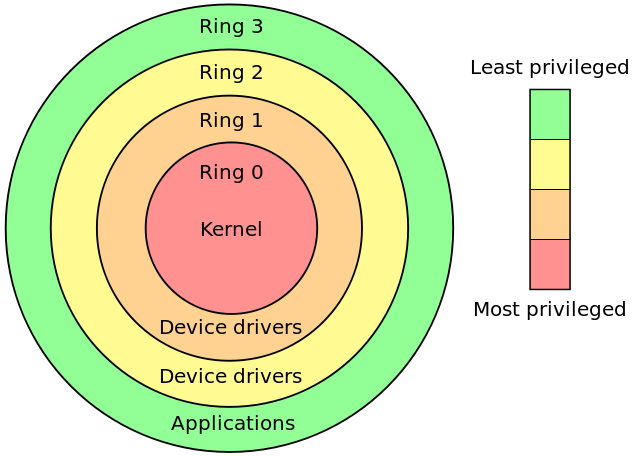
\includegraphics[width=5cm]{protection_ring.png}
\end{figure}

Trong họ vi xử lý x86, có tổng cộng 4 mức đặc quyền, được đánh số từ 0 cho đến 3. Mức 0 là mức có đặc quyền cao nhất. Nhưng hầu hết các nhân hệ điều hành cho x86 như Windows, Linux chỉ sử dụng hai mức đặc quyền là mức 0 và mức 3. Hai mức 0 và 3 đó thường được gọi lần lượt là kernel mode và user mode. Kernel mode chỉ được sử dụng bởi nhân (kernel) của hệ điều hành, còn user mode chủ yếu trong thời gian hoạt động của các tiến trình thông thường.

Có khoảng 15 instruction (lệnh của CPU), chỉ được sử dụng ở mức đặc quyền 0 của CPU \cite{x86-rings}. Có nhiều những instruction khác thì bị giới hạn  trong các toán hạng của nó khi ở ngoài mức 0. Ví dụ các thanh ghi segment không thể được set ở user mode. Những instruction chỉ được sử dụng ở mức đặc quyển 0 đó có thể phá vỡ cơ chế bảo vệ hoặc gây nên xáo trộn trong hệ thống nếu được phép sử dụng ở user mode.

\section{Phân đoạn trong phần cứng x86}
Bắt đầu từ phiên bản 80286, Trong vi xử lý Intel có tồn tại hai cách để thực hiện dịch địa chỉ đó là \textit{real mode} và \textit{protected mode}. Real mode tồn tại chủ yếu để duy trì tính tương thích ngược đối với những thế hệ vi xử lý cũ và để cho phép hệ điều hành có thể khởi động. \cite{address_translation}

Trong protected mode, địa chỉ tồn tại dưới 3 dạng:
\begin{itemize}
\item Địa chỉa logic: Địa chỉ tồn tại dưới dạng \textit{segment:offset}, là địa chỉ được CPU được sử dụng bên trong, trước khi qua khối phân đoạn. 
\item Địa chỉ tuyến tính: Địa chỉ được tạo từ địa chỉ logic sau khi qua quá trình phân đoạn và trước khi qua quá trình phân trang. 
\item Địa chỉ vật lý: Là địa chỉ được truyền ra ngoài CPU tới các thành phần khác trong hệ thống (Ví dụ RAM).
\end{itemize}

\begin{figure}[h]
\centering
\caption{Quá trình dịch địa chỉ trong x86}
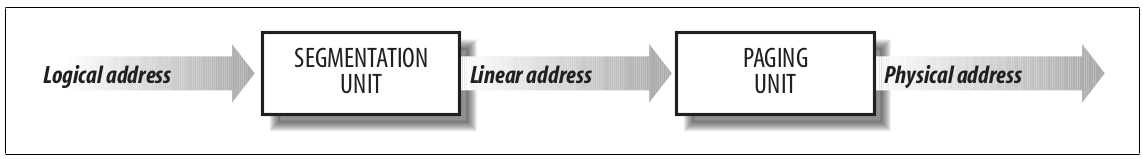
\includegraphics[width=\textwidth]{address_translation.png}
\end{figure}

\subsection{Các thanh ghi chỉ định đoạn và bảng quản lý đoạn.}
Địa chỉ logic gồm hai phần \textit{segment} và \textit{offset}, phần \textit{segment} được gọi là phần chỉ định đoạn, gồm 16 bit. Được chia thành các phần như mô tả trong hình: 
\begin{figure}[h]
\centering
\caption{Định dạng của \textit{segment}}
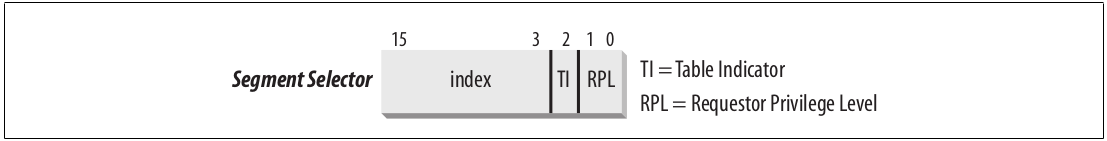
\includegraphics[width=\textwidth]{segment_selector.png}
\end{figure}

Hai thành phần chính trong cơ chế phân đoạn của x86 là các thanh ghi segment 16 bit như cs (code segment), ds (data segment), ss (stack segment),... và bảng quản lý đoạn. Có hai bảng quản lý đoạn: Global Descriptor Table (GDT) và Local Descriptor Table (LDT), nằm trong bộ nhớ chính, địa chỉ của chúng được quản lý bởi hai thanh ghi gdtr và ldtr. Bit TI trong mỗi thanh ghi segment chỉ định bảng nào sẽ được lựa chọn, bằng 0 nếu như đang sử dụng GDT, bằng 1 là LDT. Phần index là chỉ số của phần tử tương ứng nằm trong bảng quản lý đoạn. 

RPL: Requestor Privilege Level: Chỉ định mức độ đặc quyền hiện tại khi thanh ghi cs được nạp. 

Mỗi phần tử trong bảng quản lý đoạn có 8 byte, được chia thành nhiều trường như sau: 
\begin{itemize}
\item Base: 32 bit; Chứa địa chỉ tuyến tính của byte đầu tiên trong đoạn. 
\item G - granularity flag: Gồm 1 bit; nếu nó bằng 0, kích thước của đoạn được thể hiện dưới dạng byte; ngược lại, kích thước được thể hiện dưới dạng số nguyên lần của 4096 byte. 
\item Limit: 20 bit; Giới hạn của đoạn, có thể biểu diễn $2^{10}$ giá trị, nếu G = 0 thì đoạn đó có kích thước lớn nhất là 1MB; ngược lại, đoạn có kích thước lớn nhất là 4GB.
\item S: System flag; 1 bit; Nếu nó bằng 0, segment chứa các dữ liệu quan trọng như LDT; Ngược lại, nó chứa những dữ liệu thông thường. 
\item Type: 4 bit; Chỉ định loại segment và quyền truy cập.
\item DPL: 2 bit; Descriptor Privilege Level: Mức độ đặc quyền của Segment; 
\item P: 1 bit; Segment Present Flag; Nếu nó bằng 0: segment chưa được nằm trong bộ nhớ; Ngược lại, segment đã nằm trong bộ nhớ chính. 
\item D or B: 1 bit; Có giá trị bằng 1 nếu 	segment sử dụng offset là 32 bit; Ngược lại offset là 16 bit.
\item AVL: Hầu hết không được sử dụng. 
\end{itemize}

\begin{figure}[h]
\centering
\caption{Định dạng của một phần tử trong bảng quản lý đoạn chứa code (Segment Descriptor)}
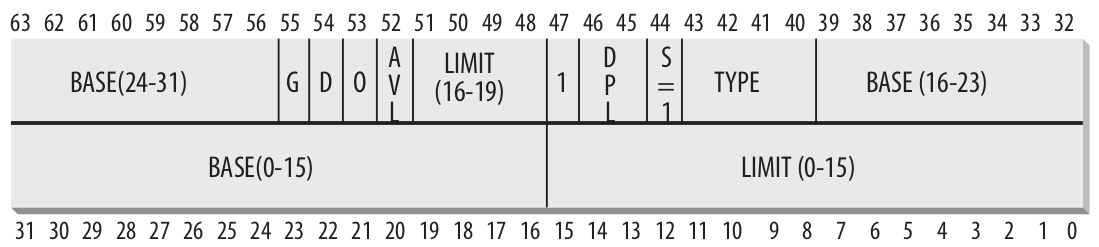
\includegraphics[width=\textwidth]{code_segment.png}
\end{figure}

\begin{figure}[h]
\centering
\caption{Mối quan hệ của các mức độ đặc quyền}
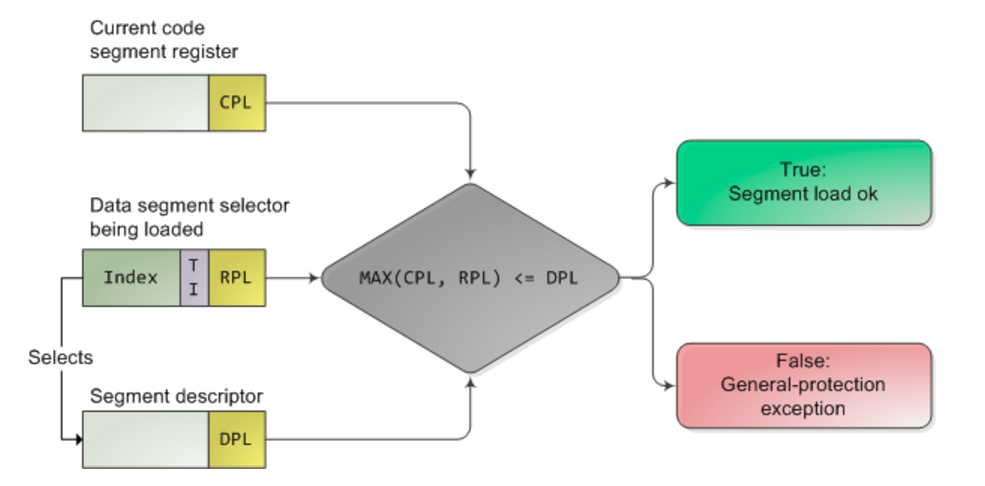
\includegraphics[width=12cm]{plevel.png}
\end{figure}

Các đoạn trong x86 thuộc một trong các loại sau:
\begin{itemize}
\item Code Segment: Đoạn đó chứa code.
\item Data Segment: Đoạn đó chứa dữ liệu. 
\item Task State Segment: Đoạn đó chứa một dữ liệu đặc biệt. Ví dụ như khi CPU hoán đổi tử User Mode sang Kernel Mode, nó nạp địa chỉ của Kernel Mode stack từ Task State Segment. TSS có thể chứa các thông tin: \cite{task_state_segment}
\begin{itemize}
\item Trạng thái các thanh ghi của vi xử lý. 
\item Quyền truy cập của các port IO. 
\item Con trỏ tới stack. 
\item Link tới TSS trước đó. 
\end{itemize}
\end{itemize}

\subsection{Truy cập nhanh đến các phần tử trong bảng quản lý đoạn.}
Một địa chỉ logic gồm 16 bit chỉ đoạn và 32 bit độ lệch (offset). Do để biết được địa chỉ bắt đầu của đoạn, ta cần truy cập đến các phần tử trong bảng quản lý đoạn, như vậy mỗi lần truy cập bộ nhớ sẽ mất thời gian gấp đôi. Để tăng tốc, họ vi xử lý 80x86 cung cấp thêm một thanh ghi đặc biệt, thanh ghi không thể được lập trình - không thể được set giá trị bởi các instruction, chứa định giá trị của các phần tử trong bảng quản lý đoạn (8 byte). Một khi các thanh ghi segment (16 bit) được set một giá trị mới, các thanh ghi 8 byte này sẽ được set giá trị của phần tử 8 byte trong bảng quản lý đoạn tương ứng với segment đó. 

\begin{figure}[h]
\centering
\caption{Cơ chế truy cập nhanh đến bảng quản lý đoạn trong x86}
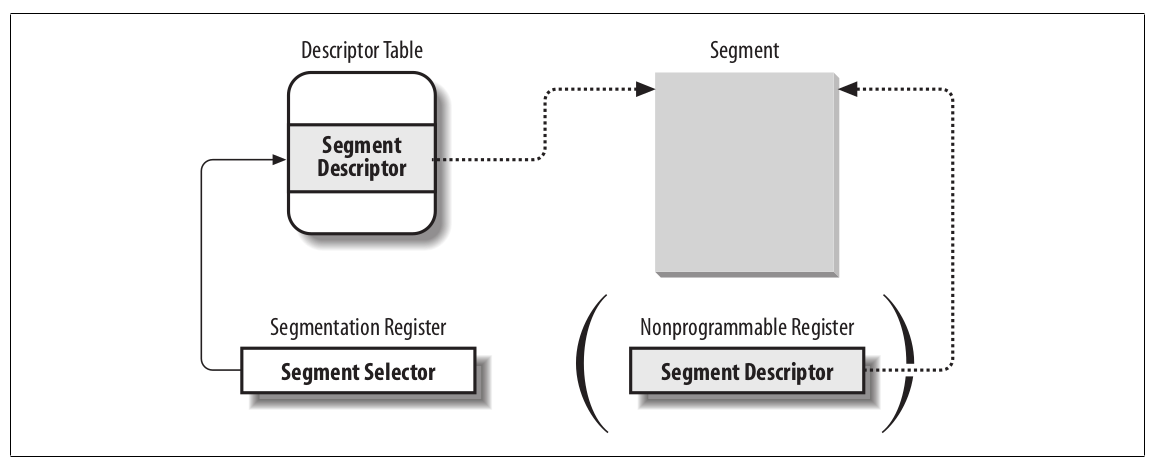
\includegraphics[width=\textwidth]{fast_access_gdt.png}
\end{figure}

\bibliographystyle{plain}

\subsection{Khối thực hiện phân đoạn}
Mỗi khi có truy cập đến bộ nhớ, khối thực hiện phân đoạn trong CPU x86 thực hiện các nhiệm vụ sau: 
\begin{itemize}
\item Xác định trường TI trong thanh ghi chỉ định đoạn, lựa chọn gdtr hoặc ldtr tương ứng. 
\item Tính toán địa chỉ của phần tử tương ứng trong bảng quản lý đoạn từ phần index trong thanh ghi chỉ định đoạn. 
\item Cộng độ lệnh (offset) của địa chỉ logic với trường base trong phần tử của bảng quản lý đoạn tương ứng. Kiểm tra các điều kiện truy cập như của Cờ P, trường limit, DPL,...
\end{itemize}

\begin{figure}[h]
\centering
\caption{Quá trình dịch địa chỉ logic.}
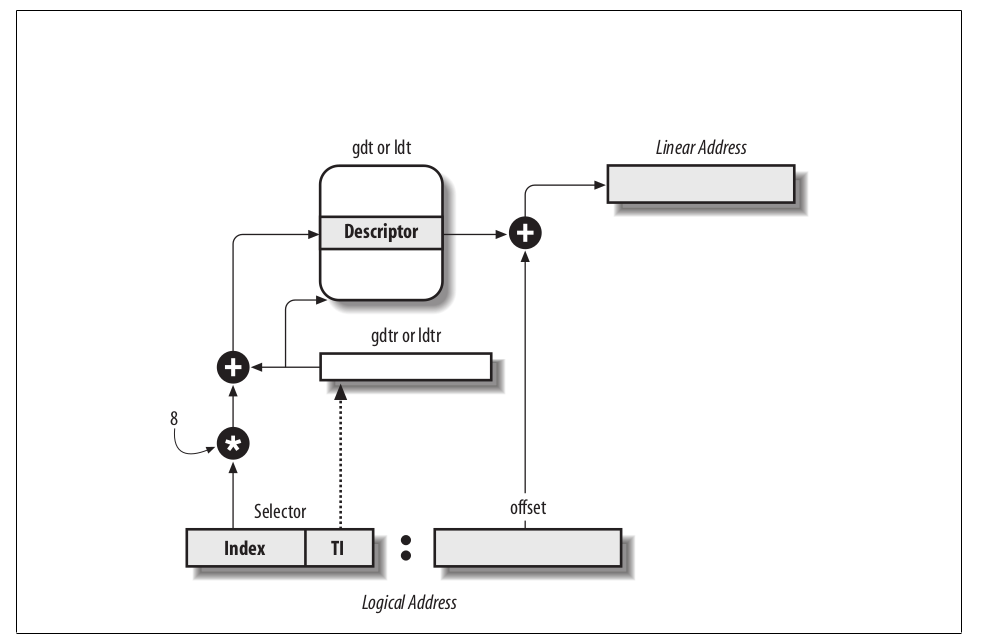
\includegraphics[width=\textwidth]{logic_translate.png}
\end{figure}

\section{Phân trang trong phần cứng x86}
Trong mỗi CPU x86 tồn tại một thành phần gọi là khối thực hiện phân trang - dịch địa chỉ tuyến tính sang địa chỉ vật lý. Nó được kích hoạt khi mà cờ PG trong thanh ghi cr0 được set giá trị 1. 

32 bit của địa chỉ tuyến tính được tách thành 3 phần:
\begin{itemize}
\item Directory: Thư mục trang: 10 bit cao nhất trong 32 bit địa chỉ tuyến tính. 
\item Table: Bảng trang: 10 bit nằm giữa.
\item Offset: Độ lệch: 12 bit thấp nhất. 
\end{itemize} 

Việc dịch địa chỉ tuyến tính thành địa chỉ vật lý được thực hiện qua 2 bước, mỗi bước ứng với một bảng dịch địa chỉ. Bảng dịch địa chỉ đầu tiên gọi là Bảng thư mục trang, bảng thứ hai được gọi là Bảng trang. Địa chỉ vật lý của bảng thư mục trang được lưu trong thanh ghi cr3.

Mục đích của việc sử dụng cơ chế phân trang 2 mức đó là làm giảm yêu cầu bộ nhớ để lưu trữ các bảng trang cho mỗi tiến trình. Mỗi một tiến trình đang chạy phải có một bảng thư mục trang gắn với nó. Tuy nhiên, không cần thiết phải luôn có bảng trang cho tiến trình tại thời điểm bắt đầu chạy. Có thể cấp phát bảng trang chỉ khi mà tiến trình đó cần đến.

Địa chỉ vật lý của bảng thư mục trang được lưu trong thanh ghi cr3. Mỗi một phần tử trong bảng thư mục trang sẽ xác định địa chỉ vật lý của bảng trang. Tương tự, mỗi phần tử trong bảng trang sẽ xác định địa chỉ vật lý của khung trang tương ứng. Trường xác định bảng thư mục trang và bảng trang đều là 10 bit. Vì vậy nên số lượng phần tử lớn nhất trong mỗi bảng là 1024. Đồng thời kích thước của mỗi trang là 4KB.

Mỗi một phần tử trong bảng thư mục trang và bảng trang là 32 bit. 20 bit cao để xác định địa chỉ vật lý của bảng trang (đối với bảng thư mục trang) hoặc địa chỉ vật lý của trang (đối với bảng trang). 12 bit thấp chứa các cờ sau: 
\begin{itemize}
\item Present: Nếu nó bằng 1, trang đã nằm trong bộ nhớ (đối với bảng trang) hoặc bảng trang đã nằm trong bộ nhớ (đối với phần tử trong bảng thư mục trang); ngược lại, bằng 0 nếu nó không tồn tại trong bộ nhớ. Khi đó nếu truy cập đến page này sẽ gây ra một ngoại lệ có tên Page Fault. 
\item Accessed: Được set giá trị 1 mỗi khi khối phân trang truy cập vào trang đó (đối với phần tử của bảng trang) hoặc mỗi khi truy cập bảng trang (đối với phần tử của bảng thư mục trang).
\item Dirty: Chỉ có trên bảng trang. Nó được set bằng 1 mỗi khi có phép toán ghi xảy ra lên trang đó. 
\item Read/Write: Nếu nó bằng 0, trang chỉ đọc; Ngược lại, trang có thể đọc và ghi.
\item PCD và PWT: Kiểm soát cơ chế cache lên trang đó. 
\item Page Size: Chỉ có trên bảng thư mục trang. Nó được set giá trị 1 trong trường hợp mỗi trang là 4MB thay vì 4KB (Khi xả ra phân trang mở rộng).
\item Global: Chỉ có trên bảng trang. Ngăn ngừa việc trang đó thường xuyên bị đẩy lên TLB (Translation Lookaside Buffers).
\end{itemize}

\begin{figure}[h]
\centering
\caption{Quá  trình dịch địa chỉ tuyến tính.}
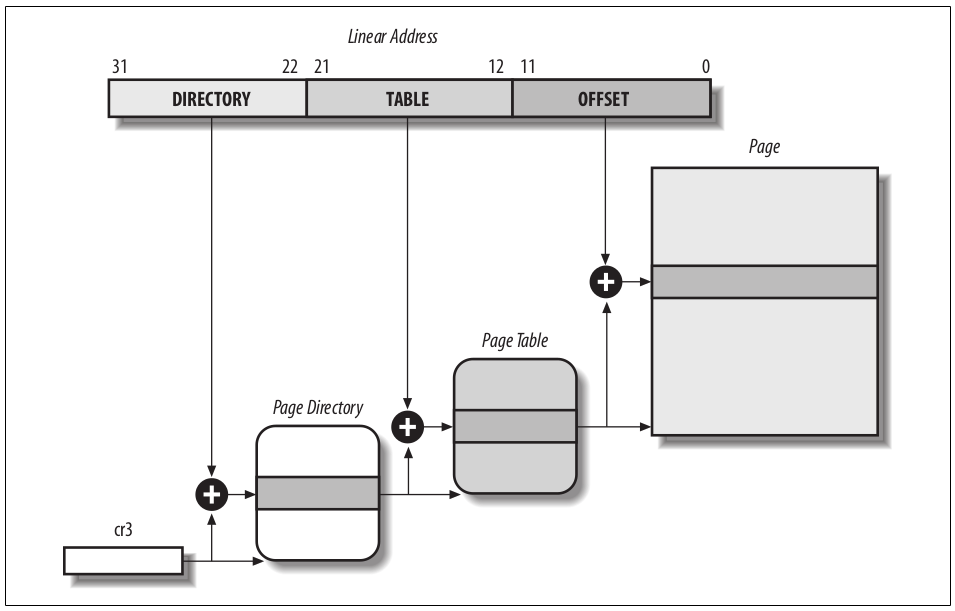
\includegraphics[width=\textwidth]{paging.png}
\end{figure}

\bibliography{refs}
\end{document}
